\chapter{Theoretical background} \label{ch:theory}

\section{Notations}

Common notations for the ship's pose, velocity and control input based on SNAME \parencite{fossen2011} are given in Table \ref{table:vessel_notations}. The pose, velocity and control input of the ship are advantageously collected in $\boldsymbol{\eta} = [x,y,\psi]^T$, $\boldsymbol{\nu} = [u,v,r]^T$ and $\boldsymbol{\tau} = [X,Y,N]^T$, respectively. It should be emphasized that pose is given relative to a North-East-Down (NED) reference frame, and velocity and control input are given in the body, i.e.\ ship's, frame \parencite{fossen2011}. That means that pose is the absolute position and orientation in a two dimensional tangent on the Earth surface oriented towards north, while velocity and control input is relative to the orientation of the ship. 

\begin{table}[H]
\centering
\begin{tabular}{ c P{2cm} P{2cm} P{2cm}  } 
 \hline
  & \textbf{Forces and moments} &  \textbf{Linear and angular velocities} &  \textbf{Positions and Euler angle}  \\ \hline
 Motion in x-direction (surge) & \gls{X} & \gls{u} &  \gls{x} \\ 
 Motion in y-direction (sway) & \gls{Y} & \gls{v} & \gls{y} \\ 
 Rotation about z-axis (yaw) & \gls{N} & \gls{r} & \gls{psi} \\ \hline
\end{tabular}
\caption{Notations for vessel. Based on SNAME (1950) \parencite{fossen2011}.}
\label{table:vessel_notations}
\end{table}

\begin{figure}[H]
    \centering
    \includegraphics[width=0.5\textwidth]{fig/ship_notations}
    \caption{Illustrations of a 6-DOF ship. From \parencite{fossen2011}.}
    \label{fig:ship_notation}
\end{figure}

\section{Ship system model}

\subsection{Ship types}

It is of relevance to concern planning with larger ships such as ferries and cargo ships. However, based on the terrain of the norwegian coast line, smaller ferries are more flexible to make different routes. 

\subsection{Marine craft}
A general ship model in both three and six degrees of freedom (\gls{dof}) is presented in \parencite{fossen2011}. For path-planning on a two dimensional map, the 3-DOF model is sufficient, such that only forward motion, sideway motion and rotational motion need to be considered, i.e.\ surge, sway and yaw respectively.



That means that the simplification of only considering a NED reference frame is not valid for global path-planning around the globe. However, global path-planning considered in this project is more local because only areas are considered, and thus the model is sufficient. Then we have that \gls{x} is the position in north direction, \gls{y} is the position in east direction, \gls{psi} is the heading angle of the ship relative to north, \gls{u} is the surge velocity, \gls{v} is the sway velocity, \gls{r} is the yaw angular velocity, \gls{X} is the surge force, \gls{Y} is the sway force and \gls{N} is the moment about the z-axis. In addition, the total speed of the ship is defined as $U=\sqrt{u^2+v^2}$. The course angle $\chi$ is defined as the angle of the velocity vector relative to north, and the sideslip $\beta$ is defined as the angle between the ship's heading and course $\chi = \psi + \beta$. With this model, rotations from body frame to NED frame are carried out utillizing the rotational matrix
\begin{equation}
\boldsymbol{R}(\psi) = \begin{bmatrix} 
\cos\psi &-\sin\psi & 0 \\
\sin\psi & \cos\psi & 0 \\
0 & 0 & 1
\end{bmatrix}.
\end{equation}



Instead of a disturbance acting on the actuation, ocean currents are considered as a velocity reference $\boldsymbol{\nu}_c^n \in \mathbb{R}^3$ in NED, such that $\boldsymbol{\nu}_r(t) = \boldsymbol{\nu}(t) - \boldsymbol{\nu}_c(t)$ where 

\begin{equation}
\boldsymbol{\nu}_c(t) = \boldsymbol{R}^T(\psi(t)) \boldsymbol{\nu}_c^n.
\end{equation}

 Wind and wave disturbances are not considered for this analysis.

The resulting kinematics and kinetics are then given by
\begin{subequations} 
	\begin{align}
	\dot{\boldsymbol{\eta}} &= \boldsymbol{R}(\psi)\boldsymbol{\nu} \\ 
	\boldsymbol{M}\dot{\boldsymbol{\nu}_r}+\boldsymbol{C}(\boldsymbol{\nu}_r)\boldsymbol{\nu}_r + \boldsymbol{D}(\boldsymbol{\nu}_r)\boldsymbol{\nu}_r  &= \boldsymbol{\tau}
	\end{align}
\end{subequations}
where $\boldsymbol{M}$, $\boldsymbol{C}(\boldsymbol{\nu})$ and $\boldsymbol{D}(\boldsymbol{\nu})$ are model matrices denoted inertia, Coriolis and damping, respectively.
A disadvantage of using these simplified dynamics is that they may be inaccurate in harsh sea state, e.g.\ high waves, when roll and pitch are no longer approximately zero. 

For simulating the ship dynamics, the states are transformed to state-space form
\begin{equation}
	\label{eq:x_dot}
	\dot{\boldsymbol{x}} = \boldsymbol{f}(\boldsymbol{x}, \boldsymbol{\tau}) = \begin{bmatrix}
		\boldsymbol{R}(\psi)\boldsymbol{\nu} \\
		\boldsymbol{M}^{-1}(\boldsymbol{\tau}  - \boldsymbol{C}(\boldsymbol{\nu}_r)\boldsymbol{\nu}_r - \boldsymbol{D}(\boldsymbol{\nu}_r)\boldsymbol{\nu}_r) + \dot{\boldsymbol{\nu}}_c
	\end{bmatrix}
\end{equation}
where $\boldsymbol{x}= [\boldsymbol{\eta}^T, \boldsymbol{\nu}^T]^T$.



\section{Scenarios}
Coastal areas in Norway. Possibilities: Haugesund-Bergen, Bergen-Førde, Byfjorden-Førde, nord for Trondheim og Kristiansund. Particularly: Eldøy-Mongstad.

\begin{figure}[H]
\centering
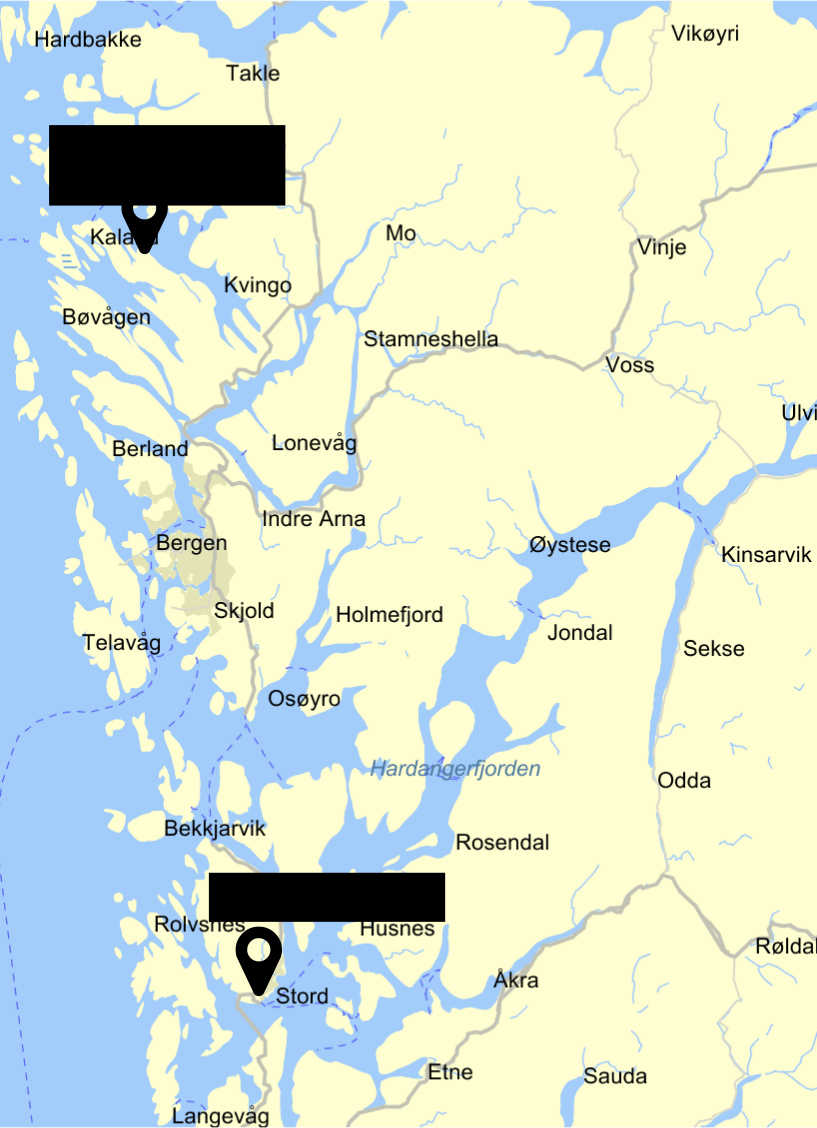
\includegraphics[width=0.7\textwidth]{fig/scenario}
\label{fig:scenario}
\caption{Scenario: Route planning from Eldøy to Mongstad}
\label{fig:scenario}
\end{figure}


\section{Validation}
\subsection{Kongsberg Maritime ECDIS}
Kongsberg ECDIS is an industrial validation system.

\subsection{Rules}


\section{Benchmarking}
\subsection{Kongsberg Digital Maritime Simulator}
K-SIM is a maritime industrial simulator used for verification. 

\subsection{Performance metrics}
\begin{itemize}
  \item Time complexity
  \item Memory complexity
  \item Travel time
  \item Energy consumption
  \item Actuator wear and tear
  \item Robustness to uncertainty
  \item Repeatability
  \item Human predictability
  \item (Passenger comfort)
  \item Tunability
\end{itemize}

Travel time is measured as
\begin{equation}
	f_t = t_f - t_0
\end{equation}
where $t_f$ is the final time and $t_0$ is the start time.

Energy consumption is measured as
\begin{equation}
	\label{eq:metric_energy}
	f_e = \int_{t_0}^{t_f} |\boldsymbol{\tau}(t)|^T|\boldsymbol{\nu}(t)|dt
\end{equation}
where $\boldsymbol{\tau}$ is the actuation, $\boldsymbol{\nu}$ is the velocity, $t_0$ is the start time and $t_f$ is the end time. 


Actuator wear and tear is measured as
\begin{equation}
	\label{eq:metric_actuator}
	f_a = \int_{t_0}^{t_f} |\dot{\bar{\tau}}(t)| dt
\end{equation}
where $\bar{\tau}(t) = \sqrt{X(t)^2+N(t)^2}$.

